\documentclass[12pt,a4paper]{article}

% ─── Page Layout ───────────────────────────────────────────────────────────────
\usepackage[a4paper, margin=0.8in, headheight=14pt]{geometry}

% ─── Fonts (XeLaTeX) ───────────────────────────────────────────────────────────
\usepackage{fontspec}
\usepackage{unicode-math}
\setmainfont{TeX Gyre Pagella}
\setmonofont[Scale=0.88]{TeX Gyre Cursor}
\setmathfont{Latin Modern Math}

% ─── Packages ──────────────────────────────────────────────────────────────────
\usepackage{xcolor}
\usepackage{colortbl}
\usepackage{titlesec}
\usepackage{enumitem}
\usepackage{tabularx}
\usepackage{booktabs}
\usepackage{array}
\usepackage{amsmath}
\usepackage{tikz}
\usetikzlibrary{shapes.geometric, arrows.meta, positioning, calc, fit, decorations.pathreplacing}
\usepackage{tcolorbox}
\tcbuselibrary{skins, breakable}
\usepackage{hyperref}
\usepackage{fancyhdr}
\usepackage{graphicx}
\usepackage{microtype}
\hyphenpenalty=10000
\exhyphenpenalty=10000
\sloppy
\usepackage{caption}
\usepackage{setspace}
\usepackage{multirow}
\usepackage{tocloft}

% ─── Q&A helper ────────────────────────────────────────────────────────────────
\newcommand{\Q}[1]{\textbf{#1}\par\noindent\ignorespaces}

% ─── Colour Palette ────────────────────────────────────────────────────────────
\definecolor{myred}{RGB}{196,30,58}
\definecolor{mydark}{RGB}{30,30,50}
\definecolor{mygreen}{RGB}{14,120,80}
\definecolor{myteal}{RGB}{0,130,140}
\definecolor{myamber}{RGB}{180,100,0}
\definecolor{mypurple}{RGB}{100,30,160}
\definecolor{mygray}{RGB}{246,247,249}
\definecolor{mgframe}{RGB}{180,185,200}
\definecolor{watermark}{RGB}{145,150,170}
\definecolor{hdrred}{RGB}{250,232,235}
\definecolor{hdrgreen}{RGB}{220,244,233}
\definecolor{hdrteal}{RGB}{220,242,244}
\definecolor{hdramber}{RGB}{253,242,215}
\definecolor{hdrpurple}{RGB}{238,228,255}
\definecolor{hdrgray}{RGB}{238,240,245}
\definecolor{rowalt}{RGB}{250,251,253}

% ─── Section Formatting ────────────────────────────────────────────────────────
\titleformat{\section}
  {\large\bfseries\color{myred}}{\thesection.}{0.5em}{}
  [\vspace{1pt}{\color{myred}\rule{\linewidth}{0.8pt}}]
\titleformat{\subsection}
  {\normalsize\bfseries\color{myteal}}{\thesubsection}{0.5em}{}
\titlespacing*{\section}{0pt}{18pt}{7pt}
\titlespacing*{\subsection}{0pt}{11pt}{4pt}

% ─── Paragraph ─────────────────────────────────────────────────────────────────
\setlength{\parindent}{0pt}
\setlength{\parskip}{4pt}

% ─── TOC Styling ───────────────────────────────────────────────────────────────
\renewcommand{\cfttoctitlefont}{\large\bfseries\color{myred}}
\renewcommand{\cftaftertoctitle}{\par\noindent{\color{myred}\rule{\linewidth}{0.8pt}}}
\setlength{\cftbeforetoctitleskip}{0pt}
\setlength{\cftaftertoctitleskip}{6pt}
\renewcommand{\cftsecfont}{\normalsize\bfseries\color{mydark}}
\renewcommand{\cftsecpagefont}{\normalsize\bfseries\color{mydark}}
\renewcommand{\cftsecleader}{\cftdotfill{\cftdotsep}}
\setlength{\cftbeforesecskip}{7pt}
\renewcommand{\cftsubsecfont}{\small\color{mydark}}
\renewcommand{\cftsubsecpagefont}{\small\color{mydark}}
\setlength{\cftbeforesubsecskip}{3pt}
\setlength{\cftsubsecindent}{1.4em}

% ─── Table helpers ─────────────────────────────────────────────────────────────
\renewcommand{\arraystretch}{1.45}
\setlength{\tabcolsep}{6pt}
\arrayrulecolor{mydark}
\newcolumntype{B}[1]{>{\small\bfseries\raggedright\arraybackslash}m{#1}}
\newcolumntype{Y}{>{\small\raggedright\arraybackslash}X}
\renewcommand{\tabularxcolumn}[1]{m{#1}}

% ─── Header / Footer ───────────────────────────────────────────────────────────
\pagestyle{fancy}
\fancyhf{}
\fancyhead[L]{\small\color{myred}\textbf{PE-EC702B}\;\color{mydark}--- Digital Image and Video Processing}
\fancyhead[R]{\small\color{myteal}\textbf{Module 5 Notes}}
\fancyfoot[C]{\small\color{mydark}\thepage}
\fancyfoot[R]{\small\color{watermark}\textit{\copyright\ Biraj}}
\renewcommand{\headrulewidth}{0.5pt}
\renewcommand{\footrulewidth}{0.3pt}

% ─── Hyperref ──────────────────────────────────────────────────────────────────
\hypersetup{
  colorlinks=true, linkcolor=myteal, urlcolor=myteal,
  pdfauthor={Biraj Sarkar},
  pdftitle={PE-EC702B --- Module 5 Notes}
}

% ─── tcolorbox styles ──────────────────────────────────────────────────────────
\tcbset{
  tikzbox/.style={
    colback=mygray, colframe=mgframe, boxrule=0.6pt, arc=4pt,
    left=8pt, right=8pt, top=6pt, bottom=6pt,
    colbacktitle=mgframe, coltitle=mydark,
    fonttitle=\small\bfseries
  },
  defbox/.style={
    colback=hdrgreen, colframe=mygreen, boxrule=0.8pt, arc=4pt,
    left=9pt, right=9pt, top=6pt, bottom=6pt,
    colbacktitle=mygreen, coltitle=white,
    fonttitle=\small\bfseries
  },
  formulabox/.style={
    colback=hdrteal, colframe=myteal, boxrule=0.8pt, arc=4pt,
    left=9pt, right=9pt, top=7pt, bottom=7pt,
    colbacktitle=myteal, coltitle=white,
    fonttitle=\small\bfseries
  },
  examplebox/.style={
    colback=hdramber, colframe=myamber, boxrule=0.8pt, arc=4pt,
    left=9pt, right=9pt, top=6pt, bottom=6pt,
    colbacktitle=myamber, coltitle=white,
    fonttitle=\small\bfseries,
    breakable
  },
  masonbox/.style={
    colback=hdrpurple, colframe=mypurple, boxrule=0.8pt, arc=4pt,
    left=9pt, right=9pt, top=6pt, bottom=6pt,
    colbacktitle=mypurple, coltitle=white,
    fonttitle=\small\bfseries
  },
  exambox/.style={
    colback=hdrpurple, colframe=mypurple, boxrule=1pt, arc=5pt,
    left=10pt, right=10pt, top=8pt, bottom=8pt,
    colbacktitle=mypurple, coltitle=white,
    fonttitle=\bfseries,
    breakable, title after break={\textbf{Frequently Asked / Viva Questions (contd.)}}}
}
\tcbset{breakable}

% ─── TikZ styles ───────────────────────────────────────────────────────────────
\tikzset{
  block/.style={rectangle, draw=myteal, fill=hdrteal,
    text width=2.1cm, align=center, minimum height=0.85cm,
    font=\small, rounded corners=3pt, line width=0.7pt},
  arrow/.style={-Stealth, thick, color=mydark},
  line/.style={thick, color=mydark}
}

% ═══════════════════════════════════════════════════════════════════════════════
\begin{document}
% ═══════════════════════════════════════════════════════════════════════════════

\begin{center}
  {\LARGE\bfseries\color{myred} PE-EC702B --- Digital Image and Video Processing}\\[5pt]
  {\normalsize\color{mydark} Semester VII \quad$\bullet$\quad 3L:0T:0P \quad$\bullet$\quad 3 Credits}\\[3pt]
  {\normalsize\color{myteal}\textbf{Module 5 Exam Notes: Wavelets and Multi-resolution Image Processing}}\\[3pt]
  {\small\color{mydark} CGEC \;$|$\; B.Tech ECE (2023--27) \;$|$\; \textit{Biraj Sarkar}}
\end{center}
\vspace{2pt}
\noindent{\color{myred}\rule{\linewidth}{1.5pt}}
\vspace{2pt}

\hypersetup{linkcolor=mydark}
\tableofcontents
\hypersetup{linkcolor=myteal}
\newpage

% ===============================================================================
\section{Limitations of Fourier Transform}
% ===============================================================================

The Fourier Transform is highly effective at analyzing stationary signals. However, it loses all temporal information when transforming to the frequency domain.

\begin{tcolorbox}[defbox, title={Time-Frequency Limitations}]
\textbf{Uncertainty Principle (Heisenberg's):} States that one cannot simultaneously determine both the exact time location and frequency content of a signal with infinite precision:
\begin{equation}
  \Delta t \cdot \Delta f \ge \frac{1}{4\pi}
\end{equation}
where $\Delta t$ is time resolution and $\Delta f$ is frequency resolution.
\end{tcolorbox}

\subsection{STFT vs. Wavelet Transform}
\begin{itemize}[leftmargin=*, itemsep=3.5pt]
  \item \textbf{Short-Time Fourier Transform (STFT):} Uses a sliding temporal window $w(t)$ to localize frequencies.
    \begin{itemize}[leftmargin=1em, itemsep=1pt]
      \item \textit{Limitation:} The window size is fixed. A wide window yields good frequency resolution but poor time resolution, while a narrow window yields the opposite.
    \end{itemize}
  \item \textbf{Wavelet Transform:} Solves this by using variable window sizes (\textbf{Time-Frequency Localization}):
    \begin{itemize}[leftmargin=1em, itemsep=1pt]
      \item \textit{High frequencies:} Analyzed with narrow window sizes (high time resolution, coarse frequency resolution).
      \item \textit{Low frequencies:} Analyzed with wide window sizes (coarse time resolution, high frequency resolution).
    \end{itemize}
\end{itemize}

% ===============================================================================
\section{Continuous Wavelet Transform (CWT)}
% ===============================================================================

The Continuous Wavelet Transform decomposes a continuous signal into shifted and scaled versions of a prototype function $\psi(t)$ (called the \textbf{mother wavelet}).

\begin{tcolorbox}[formulabox, title={CWT Formulations}]
The CWT of a signal $f(t)$ is defined as:
\begin{equation}
  W(a,b) = \int_{-\infty}^{\infty} f(t) \psi_{a,b}^*(t) \, dt
\end{equation}
where $\psi_{a,b}(t)$ is obtained by scaling and translating the mother wavelet:
\begin{equation}
  \psi_{a,b}(t) = \frac{1}{\sqrt{|a|}} \psi\left(\frac{t - b}{a}\right)
\end{equation}
\begin{itemize}[leftmargin=*, itemsep=2.5pt]
  \item $a \in \mathbb{R} \setminus \{0\}$ is the \textbf{scale parameter} (inversely proportional to frequency).
  \item $b \in \mathbb{R}$ is the \textbf{translation parameter} (represents time shift).
  \item The mother wavelet must satisfy the \textit{admissibility condition} (zero mean): $\int_{-\infty}^{\infty} \psi(t) \, dt = 0$.
\end{itemize}
\end{tcolorbox}

% ===============================================================================
\section{Wavelet Bases and Multi-resolution Analysis (MRA)}
% ===============================================================================

Multi-resolution Analysis (MRA) structures the Hilbert space $L^2(\mathbb{R})$ into a nested sequence of approximation spaces $V_j$ and detail spaces $W_j$.

\begin{itemize}[leftmargin=*, itemsep=3.5pt]
  \item \textbf{Scaling Function $\phi(t)$:} Spans the approximation space $V_0$. Satisfies the refinement (dilation) equation:
    \begin{equation}
      \phi(t) = \sqrt{2} \sum_n h_\phi(n) \phi(2t - n)
    \end{equation}
  \item \textbf{Wavelet Function $\psi(t)$:} Spans the detail space $W_0$ (orthogonal complement: $V_1 = V_0 \oplus W_0$). Satisfies:
    \begin{equation}
      \psi(t) = \sqrt{2} \sum_n h_\psi(n) \phi(2t - n)
    \end{equation}
    where $h_\phi(n)$ and $h_\psi(n)$ are the scaling and wavelet coefficients (filters).
\end{itemize}

% ===============================================================================
\section{Subband Filter Banks}
% ===============================================================================

Discrete wavelet decomposition and reconstruction are implemented using digital filter banks.

\begin{tcolorbox}[tikzbox, title={2-Channel Subband Coder Block Diagram}]
\centering
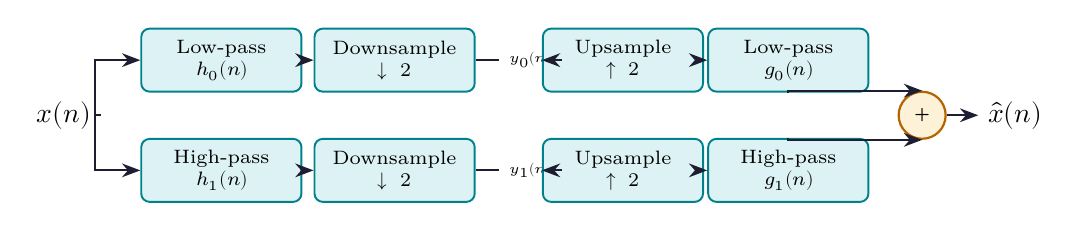
\begin{tikzpicture}[node distance=0.4cm and 0.8cm,
  sblock/.style={rectangle, draw=myteal, fill=hdrteal, text width=1.8cm,
    align=center, minimum height=0.8cm, font=\scriptsize,
    rounded corners=3pt, line width=0.7pt},
  junc/.style={circle, draw=myamber, fill=hdramber, minimum size=0.45cm,
    font=\tiny\bfseries, line width=0.8pt}]
    
  % Input
  \node (in) at (-0.5, 0) {$x(n)$};
  
  % Analysis Filters
  \node[sblock] (h0) at (1.5, 0.7) {Low-pass\\$h_0(n)$};
  \node[sblock] (h1) at (1.5, -0.7) {High-pass\\$h_1(n)$};
  \draw[arrow] (in) -- +(0.4, 0) |- (h0.west);
  \draw[arrow] (in) -- +(0.4, 0) |- (h1.west);
  
  % Downsamplers
  \node[sblock] (down0) at (3.7, 0.7) {Downsample\\$\downarrow 2$};
  \node[sblock] (down1) at (3.7, -0.7) {Downsample\\$\downarrow 2$};
  \draw[arrow] (h0) -- (down0);
  \draw[arrow] (h1) -- (down1);
  
  % Midpoints (subbands)
  \node (ch0) [right=0.3cm of down0] {\tiny $y_0(n)$};
  \node (ch1) [right=0.3cm of down1] {\tiny $y_1(n)$};
  \draw[line] (down0) -- (ch0);
  \draw[line] (down1) -- (ch1);

  % Upsamplers
  \node[sblock] (up0) at (6.6, 0.7) {Upsample\\$\uparrow 2$};
  \node[sblock] (up1) at (6.6, -0.7) {Upsample\\$\uparrow 2$};
  \draw[arrow] (ch0) -- (up0);
  \draw[arrow] (ch1) -- (up1);
  
  % Synthesis Filters
  \node[sblock] (g0) at (8.7, 0.7) {Low-pass\\$g_0(n)$};
  \node[sblock] (g1) at (8.7, -0.7) {High-pass\\$g_1(n)$};
  \draw[arrow] (up0) -- (g0);
  \draw[arrow] (up1) -- (g1);
  
  % Sum junction
  \node[junc] (sum) at (10.4, 0) {+};
  \draw[arrow] (g0) |- (sum.north);
  \draw[arrow] (g1) |- (sum.south);
  
  % Output
  \node (out) [right=0.4cm of sum] {$\hat{x}(n)$};
  \draw[arrow] (sum) -- (out);
\end{tikzpicture}
\end{tcolorbox}

\begin{itemize}[leftmargin=*, itemsep=3.5pt]
  \item \textbf{Analysis Bank:} Splits the signal into low-frequency approximation subband ($y_0$) and high-frequency detail subband ($y_1$). Downsampling ($\downarrow 2$) discards redundant odd samples.
  \item \textbf{Synthesis Bank:} Reconstructs the signal by upsampling ($\uparrow 2$, inserting zeros) and filtering.
  \item \textbf{Perfect Reconstruction Condition:} The filters must satisfy:
    \begin{align}
      g_0(n) &= h_0(-n), \quad g_1(n) = h_1(-n) \\
      H_0(-z)G_0(z) &+ H_1(-z)G_1(z) = 0 \quad \text{(Alias Cancellation)}
    \end{align}
  \item \textbf{Wavelet Packets:} In standard DWT, only the low-pass output is recursively decomposed. In \textbf{Wavelet Packet decomposition}, both the low-pass and high-pass branches are recursively filtered, producing a balanced tree.
\end{itemize}

% ===============================================================================
\section{Worked Examples}
% ===============================================================================

\begin{tcolorbox}[examplebox, title={1D Haar Wavelet Transform}]
\textbf{Problem:} Given a 4-point input signal $\mathbf{x} = [4, 6, 10, 12]^T$. Apply a 1-level Discrete Haar Wavelet Transform. Use the orthogonal Haar analysis filters:
\begin{align*}
  \text{Low-pass (approximation):} \quad h_0 &= \left[ \frac{1}{\sqrt{2}}, \frac{1}{\sqrt{2}} \right] \\[4pt]
  \text{High-pass (detail):} \quad h_1 &= \left[ \frac{1}{\sqrt{2}}, -\frac{1}{\sqrt{2}} \right]
\end{align*}
Compute the approximation coefficients $\mathbf{a}$ and detail coefficients $\mathbf{d}$ after downsampling.

\par\noindent\rule{\linewidth}{0.5pt}\par
\textbf{Solution:}
Discrete convolution is followed by downsampling by 2 ($\downarrow 2$). This is equivalent to applying the filters to non-overlapping pairs of input samples.

\textbf{1. Calculate Approximation Coefficients ($a_n$):}
\begin{itemize}[leftmargin=1.5em, itemsep=2.5pt]
  \item For the first pair $\{x(0), x(1)\} = \{4, 6\}$:
    \begin{equation*}
      a_0 = \frac{1}{\sqrt{2}}x(0) + \frac{1}{\sqrt{2}}x(1) = \frac{4 + 6}{\sqrt{2}} = \frac{10}{\sqrt{2}} = 5\sqrt{2} \approx 7.07
    \end{equation*}
  \item For the second pair $\{x(2), x(3)\} = \{10, 12\}$:
    \begin{equation*}
      a_1 = \frac{1}{\sqrt{2}}x(2) + \frac{1}{\sqrt{2}}x(3) = \frac{10 + 12}{\sqrt{2}} = \frac{22}{\sqrt{2}} = 11\sqrt{2} \approx 15.56
    \end{equation*}
\end{itemize}
So, the approximation coefficient vector is: $\mathbf{a} = [5\sqrt{2}, 11\sqrt{2}]^T$.

\textbf{2. Calculate Detail Coefficients ($d_n$):}
\begin{itemize}[leftmargin=1.5em, itemsep=2.5pt]
  \item For the first pair $\{4, 6\}$:
    \begin{equation*}
      d_0 = \frac{1}{\sqrt{2}}x(0) - \frac{1}{\sqrt{2}}x(1) = \frac{4 - 6}{\sqrt{2}} = \frac{-2}{\sqrt{2}} = -\sqrt{2} \approx -1.414
    \end{equation*}
  \item For the second pair $\{10, 12\}$:
    \begin{equation*}
      d_1 = \frac{1}{\sqrt{2}}x(2) - \frac{1}{\sqrt{2}}x(3) = \frac{10 - 12}{\sqrt{2}} = \frac{-2}{\sqrt{2}} = -\sqrt{2} \approx -1.414
    \end{equation*}
\end{itemize}
So, the detail coefficient vector is: $\mathbf{d} = [-\sqrt{2}, -\sqrt{2}]^T$.

\par\noindent\textbf{Final Haar Transform Output:}
The reconstructed representation is the combination of approximation and detail bands:
\begin{equation*}
  \mathbf{y} = [\mathbf{a} \mid \mathbf{d}]^T = [5\sqrt{2}, 11\sqrt{2}, -\sqrt{2}, -\sqrt{2}]^T
\end{equation*}
\end{tcolorbox}

\newpage

% ===============================================================================
% MANDATORY QUICK REVISION PAGE
% ===============================================================================
\begin{center}
  {\large\bfseries\color{myred} Quick Revision --- Module V}\\[3pt]
  {\small\color{mydark} Wavelets and Multi-resolution Image Processing $|$ PE-EC702B}
\end{center}
\noindent{\color{myred}\rule{\linewidth}{1.2pt}}
\vspace{4pt}

\begin{tcolorbox}[formulabox, title={\textbf{Key Formulas at a Glance}}]
\renewcommand{\arraystretch}{1.3}
\begin{tabularx}{\linewidth}{B{5.0cm} X}
Heisenberg Uncertainty & $\Delta t \cdot \Delta f \ge \frac{1}{4\pi}$ \\
Continuous Wavelet Transform & $W(a,b) = \int_{-\infty}^{\infty} f(t) \frac{1}{\sqrt{|a|}} \psi^*\left(\frac{t-b}{a}\right) \, dt$ \\
Scaling refinement eq. & $\phi(t) = \sqrt{2} \sum_n h_\phi(n) \phi(2t-n)$ \\
Wavelet refinement eq. & $\psi(t) = \sqrt{2} \sum_n h_\psi(n) \phi(2t-n)$ \\
Haar Scaling Coefficients & $h_\phi = \left[ \frac{1}{\sqrt{2}}, \frac{1}{\sqrt{2}} \right]$ \\
Haar Wavelet Coefficients & $h_\psi = \left[ \frac{1}{\sqrt{2}}, -\frac{1}{\sqrt{2}} \right]$
\end{tabularx}
\tcbset{colbacktitle=myteal, coltitle=white}
\end{tcolorbox}

\begin{tcolorbox}[defbox, title={\textbf{One-Line Definitions}}]
\begin{itemize}[leftmargin=*, itemsep=2.5pt, topsep=0pt]
  \item \textbf{Mother Wavelet:} A zero-mean, finite-energy prototype function $\psi(t)$ used to generate scaling bases.
  \item \textbf{MRA:} A mathematical framework that decomposes a signal into nested approximation spaces and details.
  \item \textbf{STFT:} A windowed Fourier transform that analyzes non-stationary signals using a fixed-width temporal slide.
  \item \textbf{Downsampling:} A process of discarding every alternate sample (e.g., $\downarrow 2$) to eliminate subband redundancy.
  \item \textbf{Wavelet Packets:} An expansion of DWT that decomposes both approximation and detail subbands recursively.
  \item \textbf{Admissibility Condition:} The zero-mean property required for wavelets to ensure the inverse transform exists.
\end{itemize}
\end{tcolorbox}

\begin{tcolorbox}[exambox, title={\textbf{Frequently Asked / Viva Questions}}]
\begin{enumerate}[leftmargin=*, itemsep=3.5pt, label=\arabic*.]
  \item \Q{Why is the standard Fourier Transform unsuitable for non-stationary signals?} Because it integrates over all time ($-\infty$ to $\infty$), meaning it yields spectral averages but completely loses the exact time locations of transient events.
  \item \Q{Explain the trade-off in STFT window sizing.} A wide window gives good frequency resolution but poor time resolution. A narrow window gives good time resolution but poor frequency resolution. It cannot adapt window width to frequency.
  \item \Q{How does the Wavelet Transform resolve the resolution trade-off in STFT?} It uses variable window sizes (multi-resolution): wide windows for low-frequency details (high frequency accuracy) and narrow windows for high-frequency details (high time accuracy).
  \item \Q{What are the physical roles of scaling and wavelet functions in MRA?} The scaling function $\phi(t)$ captures the low-frequency approximation of the signal, while the wavelet function $\psi(t)$ captures the high-frequency detail (edges).
  \item \Q{What is a 2-channel subband coder?} A system of filters and samplers that splits a signal into low-frequency (approximation) and high-frequency (detail) components, downsamples them, and later reconstructs them perfectly.
  \item \Q{State the perfect reconstruction (PR) condition for filter banks.} The analysis and synthesis filters must cancel aliasing caused by downsampling/upsampling ($H_0(-z)G_0(z) + H_1(-z)G_1(z) = 0$), and reconstruct the amplitude/phase without distortion.
  \item \Q{What is the difference between DWT and Wavelet Packet decomposition?} DWT decomposes only the low-pass approximation subband recursively at each level. Wavelet Packet decomposition decomposes both the low-pass and high-pass subbands recursively.
  \item \Q{State the properties of the Haar wavelet.} It is the oldest and simplest wavelet. It is discontinuous (step function), orthogonal, and has the shortest support (length 2), but has poor frequency selectivity.
  \item \Q{Why is downsampling necessary after subband filtering?} Because filtering halves the bandwidth of the signals. Downsampling by 2 eliminates the redundant samples, keeping the total number of samples constant.
  \item \Q{What is the scale parameter $a$ in CWT?} It represents scaling/stretching: small values of $a$ correspond to compressed wavelets (high frequencies), while large values of $a$ correspond to stretched wavelets (low frequencies).
\end{enumerate}
\tcbset{colbacktitle=myteal, coltitle=white}
\end{tcolorbox}

\begin{tcolorbox}[tikzbox, title={Fourier vs. STFT vs. Wavelet Transform}]
\centering
\renewcommand{\arraystretch}{1.2}
\begin{tabularx}{\linewidth}{>{\bfseries}B{3.2cm} Y Y Y}
\rowcolor{hdrgray} Feature & Fourier Transform & STFT & Wavelet Transform \\
\midrule
Time Resolution & None (infinite window) & Fixed (uniform window) & Variable (multi-resolution) \\
\rowcolor{rowalt} Window Width & Infinite & Fixed ($T$) & Decreases with frequency \\
Suitable For & Stationary signals & Quasi-stationary & Non-stationary (transients) \\
\bottomrule
\end{tabularx}
\tcbset{colbacktitle=myteal, coltitle=white}
\end{tcolorbox}

\end{document}
